\documentclass{proc}
% \documentclass{article}
% \documentclass{book}
\title{Latex Test}
\author{Michael Braine}
\usepackage{amsmath}
\usepackage{graphicx}
\usepackage{subcaption}

\begin{document}
  \maketitle
  \tableofcontents
  \listoffigures
  \newpage
  Test text knows no bounds!
  \section{Test Section}
  Where my homies at
  \subsection{Subsection}
  Structuring
  \begin{equation}
    f(x) = e^x + g(x)
  \end{equation}

  \begin{align*}
    f(x) &= e^x + g(x)\\
    f(x) - g(x) &= e^x
  \end{align*}

  \begin{align*}
    f(x) &= x^2\\
    g(x) &= \frac{1}{x}\\
    F(x) &= \int^a_b \frac{1}{3}x^3\\
    \frac{1}{\sqrt{x}}
  \end{align*}

  $\left[
    \begin{matrix}
      one & zero\\
      0 & 1
    \end{matrix}
  \right]$

  \begin{equation}
    \left[
      \begin{matrix}
        one & zero\\
        0 & 1
      \end{matrix}
    \right]
  \end{equation}

  $\left(\frac{1}{\sqrt{x}}\right)$

  \begin{figure}
    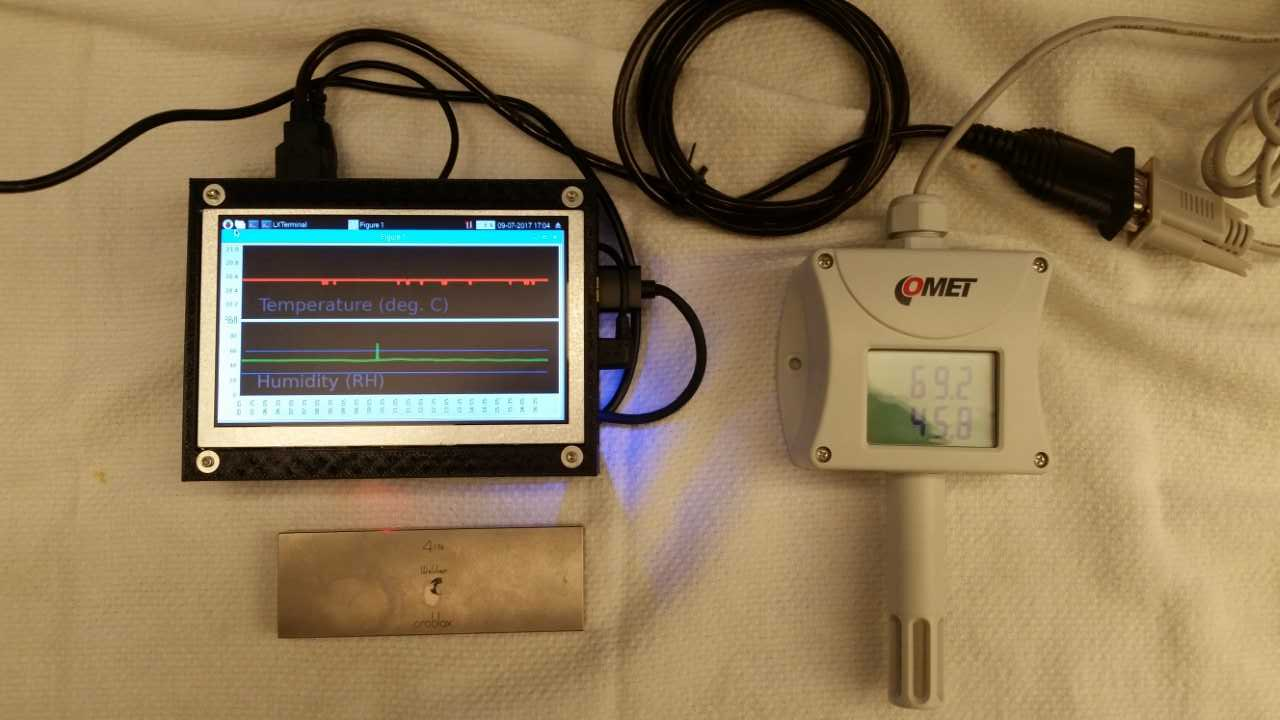
\includegraphics[width=\linewidth]{figures/index.jpeg}
    \caption{LEMAS system}
    \label{fig:LEMAS}
  \end{figure}

  As we can see in Figure \ref{fig:LEMAS}, this is the system.

  \begin{figure}
    \centering
    \begin{subfigure}{0.3\linewidth}
      
\includegraphics[width=\linewidth]{figures/fallout.jpeg}
      \caption{Mr. Fallout boy approves}
    \end{subfigure}
    \begin{subfigure}{0.5\linewidth}
      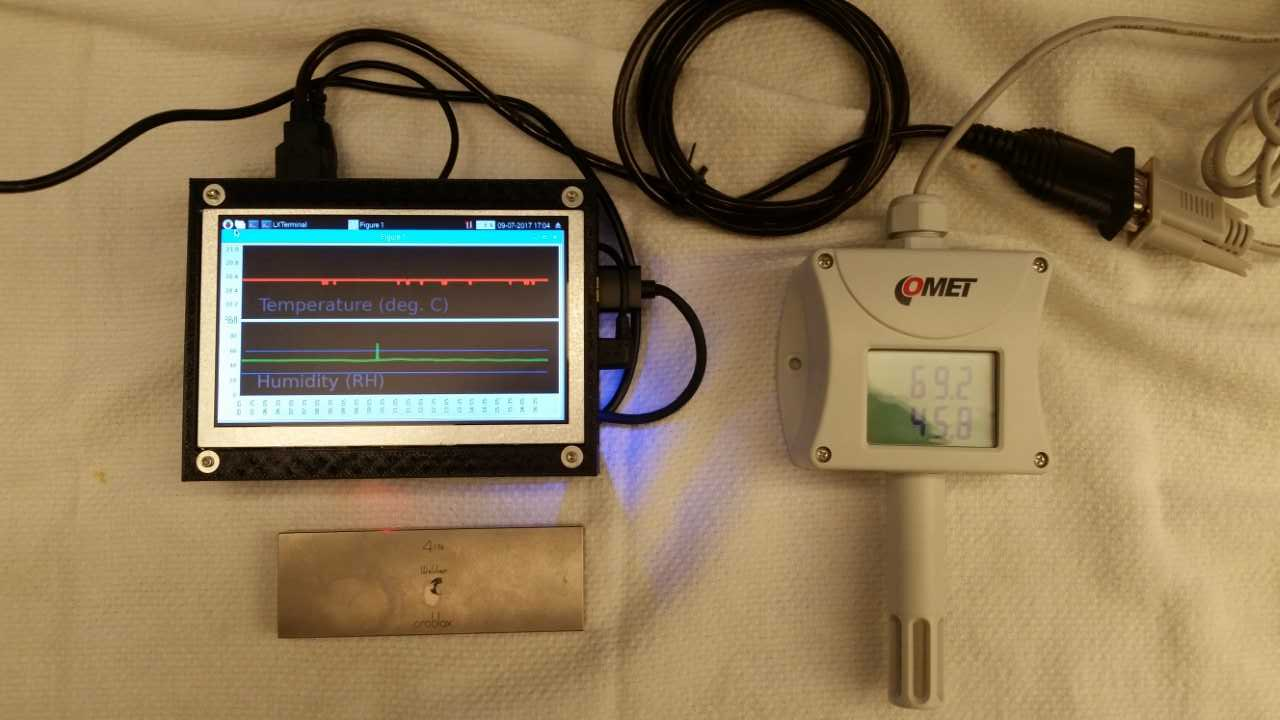
\includegraphics[width=\linewidth]{figures/index.jpeg}
      \caption{LEMAS system}
      \label{fig:2}
    \end{subfigure}
    \caption{Who approves?}
  \end{figure}

  The world doesn't revolve around itself\footnote{\label{foot1}It really doesn't}

\end{document}
